\chapter{Die Eclipse Platform}
\label{sec:EclipsePlatform}

In diesem Kapitel wird gezeigt, was Eclipse für Möglichkeiten bietet, um eine moderne Entwicklungsumgebung zu implementieren. Diese verschiedenen Möglichkeiten werden Verglichen und die Vor- und Nachteile aufgezeigt. Es werden auch die wichtigsten Eclipse Features, welche für das Entwickeln von Eclipse Rich Client Platform (RCP) Applikationen benötigt werden, beschrieben.

\section{Eclipse als Platform}

Eclipse RCP bietet eine Basis um beliebige, (nicht zwingendermassen Entwicklungsumgebungen) Betriebssystem unabhängige Applikationen zu entwickeln. Es bietet Mechanismen, wie Plugins und Extension Points, um modulares programmieren zu unterstützen und vereinfachen. Auch bietet das Framework Features, wie das Konzept von Views, Editoren und vielen mehr, welche häufig in Applikationen gebraucht werden.

\section{Plugins}

Eclipse Applikationen nützen eine auf der OSGi Speizifikation basierten Runtime. Eine Komponente in dieser Runtime ist ein Plugin. Eine Eclipse RCP Applikation besteht aus einer Ansammlung dieser Plugins. Ein Eclipse Plugin kann Extension Points \ref{extensionpointssection} anderer Plugins ansteuern und eigene Extension Points oder APIs anbieten.

\section{Extension Points}
\label{extensionpointssection}

Um Plugins erweitern zu können, bietet Eclipse das Konzept von Extension Points an. Über Extension Points können Plugins ein bestimmte Funktionalität anbieten, welches von anderen Plugins per XML deklarativ angesteuert werden kann. 
\newline
So existiert zum Beispiel ein Plugin, welches einen Extension Point für Views definiert. Andere Plugins können nun über diesen Extension Point, deklarativ in einem XML File, eine neue View erstellen und diese konfigurieren. \cite{extensionpoints}


\begin{figure}[H]
	\centering
		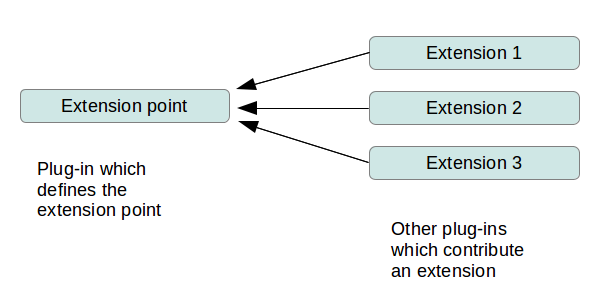
\includegraphics[scale=0.5]{platform/extensionpoint.png}
		\caption{Ein Plugin, welches einen Extension Point anbietet. Andere Plugins können diese deklarativ in einem XML File ansteuern.}
		\captionsetup{margin=0cm,font={footnotesize}}
		\label{fig:extensionpoint}
\end{figure}

Es ist auch möglich, eigene Extension Points zu definieren, falls ein Plugin für andere Entwickler offen stehen soll für Erweiterungen.

\section{Eclipse basierte MCore Entwicklungsumgebung}

Eclipse als Grundlage für eine Entwicklungsumgebung zu verwenden eignet sich besonders gut, da Eclipse schon einiges an Funktionalität für eine IDE zur Verfügung stellt und schon viele Entwicklungsumgebungen (PHP, C/C++, Pyhton, D unter anderem) als Eclipse RCP entwickelt wurden. Auch existieren einige Tools, auf welche ich noch genauer eingehen werde, wie Xtext und DLTK, welche das entwickeln einer Entwicklungsumgebung weiter vereinfachen.

\subsection{JDT}
Eine Möglichkeit die MCore Entwicklungsumgebung zu implementieren wäre die standard Features von dem Eclipse Java Development Tools (JDT) zu verwenden. Dies wäre sehr Aufwendig, da alle Features, wie Syntax Highlighting, Code Completion oder eine Outline neu implementiert werden müssten.

\subsection{XText}
XText ist ein Framework, welches es erleichtert, eine auf Eclipse basierte Entwicklungsumgebungen zu programmieren. Es ermöglicht auf schnelle Weise ein Grundgerüst einer IDE mit Features wie:

\begin{itemize} 
	\item Ein Editor mit Syntax Coloring
	\item Code Completion
	\item Compiler Integration
	\item Ein Java-basierter Debugger
	\item Eine Outline
	\item Indexing
\end{itemize}

zu generieren. \cite{xtext} Es muss lediglich eine ANTLR\cite{antlr} Grammatik für die Sprache definiert werden. Der grosse Nachteil ist, dass C, inklusive Preprozessor, zu parsen sehr schwierig ist und eine Entwicklungsumgebung somit auch mit Xtext nicht einfach zu implementieren ist.

\subsection{Dynamic Language Toolkit Framework}
Das Dynamic Language Toolkit (DLTK) ist ein weiteres Framework, welches ein Grundgerüst für eine Entwicklungsumgebungen generieren kann. Ursprünglicherweise war das Framework nur für dynamische Sprachen geignet, es kann aber auch für statische Sprachen verwendet werden. Die D Entwicklungsumgebung wurde mittels DLTK realisiert\cite{ddt}. Es bestehen aber wieder dieselben Nachteile wie bei Xtext. Da C schwierig zu parsen ist, müsste trotz dem Framework noch viel selbst implementiert werden. Da D keinen Preprozessor besitzt, konnte für diese Entwicklungsumgebung das DLTK Framework verwendet werden.

\subsection{Eclipse C/C++ Development Tools}
Das Eclipse C/C++ Development Tools (CDT), ist eine Eclipse Distribution mit Unterstützung für C und C++. Das CDT bietet alle Features, welche man von einer Entwicklungsumgebung erwartet und stellt Extension Points zur Verfügung um diese für eine eigene Entwicklungsumgebung zu gebrauchen. So kann man mit relativ wenig Aufwand einen neuen Compiler in die Entwicklungsumgebung einbinden. Dies wurde auch schon mehrfach gebraucht, um verschiende C/C++ Compiler im Eclipse CDT zu integrieren. Auf die Einbindung des Compilers wird im Kapitel \ref{compilerintegration} genauer eingegangen.

\subsection{Verwendung für MCore Eclipse}
Ich habe mich dazu entschieden, das Eclipse CDT als Target Platform zu wählen. Somit können alle Features, welche das Eclipse CDT zur Verfügung stellt, gebraucht werden. Frameworks, welche ein Grundgerüst einer Entwicklungsumgebung generieren, funktionieren nur Teilweise für C und sind somit keine guten Alternativen.
